\chapter{Linear algebra}

\devnote{This chapter is currently being written\ldots}

\dolfin{} does not have its own linear algebra data structures,
but instead uses the external libraries PETSc \cite{www:petsc}
and uBLAS \cite{www:ublas} for linear algebra functionality.

PETSc is a suite of data structures and routines for the scalable
(parallel) solution of scientific applications modeled by partial
differential equations. It employs the MPI standard for all 
message-passing communication.

uBLAS is a C++ template library that provides BLAS level 1, 2, 3
functionality (and more) for dense, packed and sparse matrices.
The design and implementation unify mathematical notation via operator
overloading and efficient code generation via expression templates.

For convenience \dolfin{} provides wrappers for some of the most
% common linear algebra functionality of PETSc and uBLAS.
For more advanced usage, \dolfin{} provides direct access to the pointers
to the underlying PETSc object that can be used with the standard PETSc 
interfaces. In the case if uBLAS-based objects, DOLFIN classes are derived
from uBLAS classes, hence the uBLAS provided functions can be used directly.


\section{PETSc}

\section{uBLAS}
%
uBLAS provides templated C++ classes for dense, unit and sparse vectors,
dense, identity, triangular, banded, symmetric, hermitian and sparse matrices. 
Views into vectors and matrices can be constructed via ranges or slices and 
adaptor classes. The library covers the usual basic linear algebra operations on
vectors and matrices: reductions like different norms, addition and subtraction 
of vectors and matrices and multiplication with a scalar, inner and outer 
products of vectors, matrix vector and matrix matrix products and triangular 
solver. The glue between containers, views and expression templated operations 
is a mostly STL conforming iterator interface.


\section{Matrices and Vectors}

\dolfin{} differentiates between sparse and dense data structures, but provides
the classes \texttt{GenericMatrix} and \texttt{GenericVector}, that define
common matrix and vector interfaces for sparse and dense data structures.

The default type \texttt{DenseMatrix} is \texttt{uBlasDenseMatrix} and the 
default type \texttt{SparseMatrix} is \texttt{uBlasSparseMatrix}. If PETSc is 
enabled, the default type \texttt{SparseMatrix} is  \texttt{PETScMatrix}. The 
corresponding vector default types are defined similarly. The default types 
\texttt{Matrix} and \texttt{Vector} are set to \texttt{SparseMatrix} and 
\texttt{SparseVector}.

\texttt{uBlasDenseMatrix} and \texttt{uBlasSparseMatrix} have
a common implementation in \texttt{uBLASMatrix}, which is a wrapper
for a Boost uBLAS matrix of type \texttt{Mat}.
The intention is to provide a uniform interface with respect to other
matrix data types in \dolfin().
For advanced usage, refer to the documentation for
uBLAS which can be found at \cite{www:ublas}.

\texttt{PETScMatrix} is a simple wrapper for the PETSc matrix
pointer \texttt{Mat}. Again the interface is intentionally simple.
For advanced usage, access the PETSc Mat pointer using the function
\texttt{mat()} and use the standard PETSc interface
\texttt{www:petsc}.
For parallel matrices, the PETSc interface has to be used directly.

Similarly, \texttt{PETScVector} and \texttt{uBLASVector} are
simple wrappers of the PETSc vector pointer \texttt{Vec} and
the Boost ublas \texttt{vector}.

\begin{figure}
  \begin{center}
    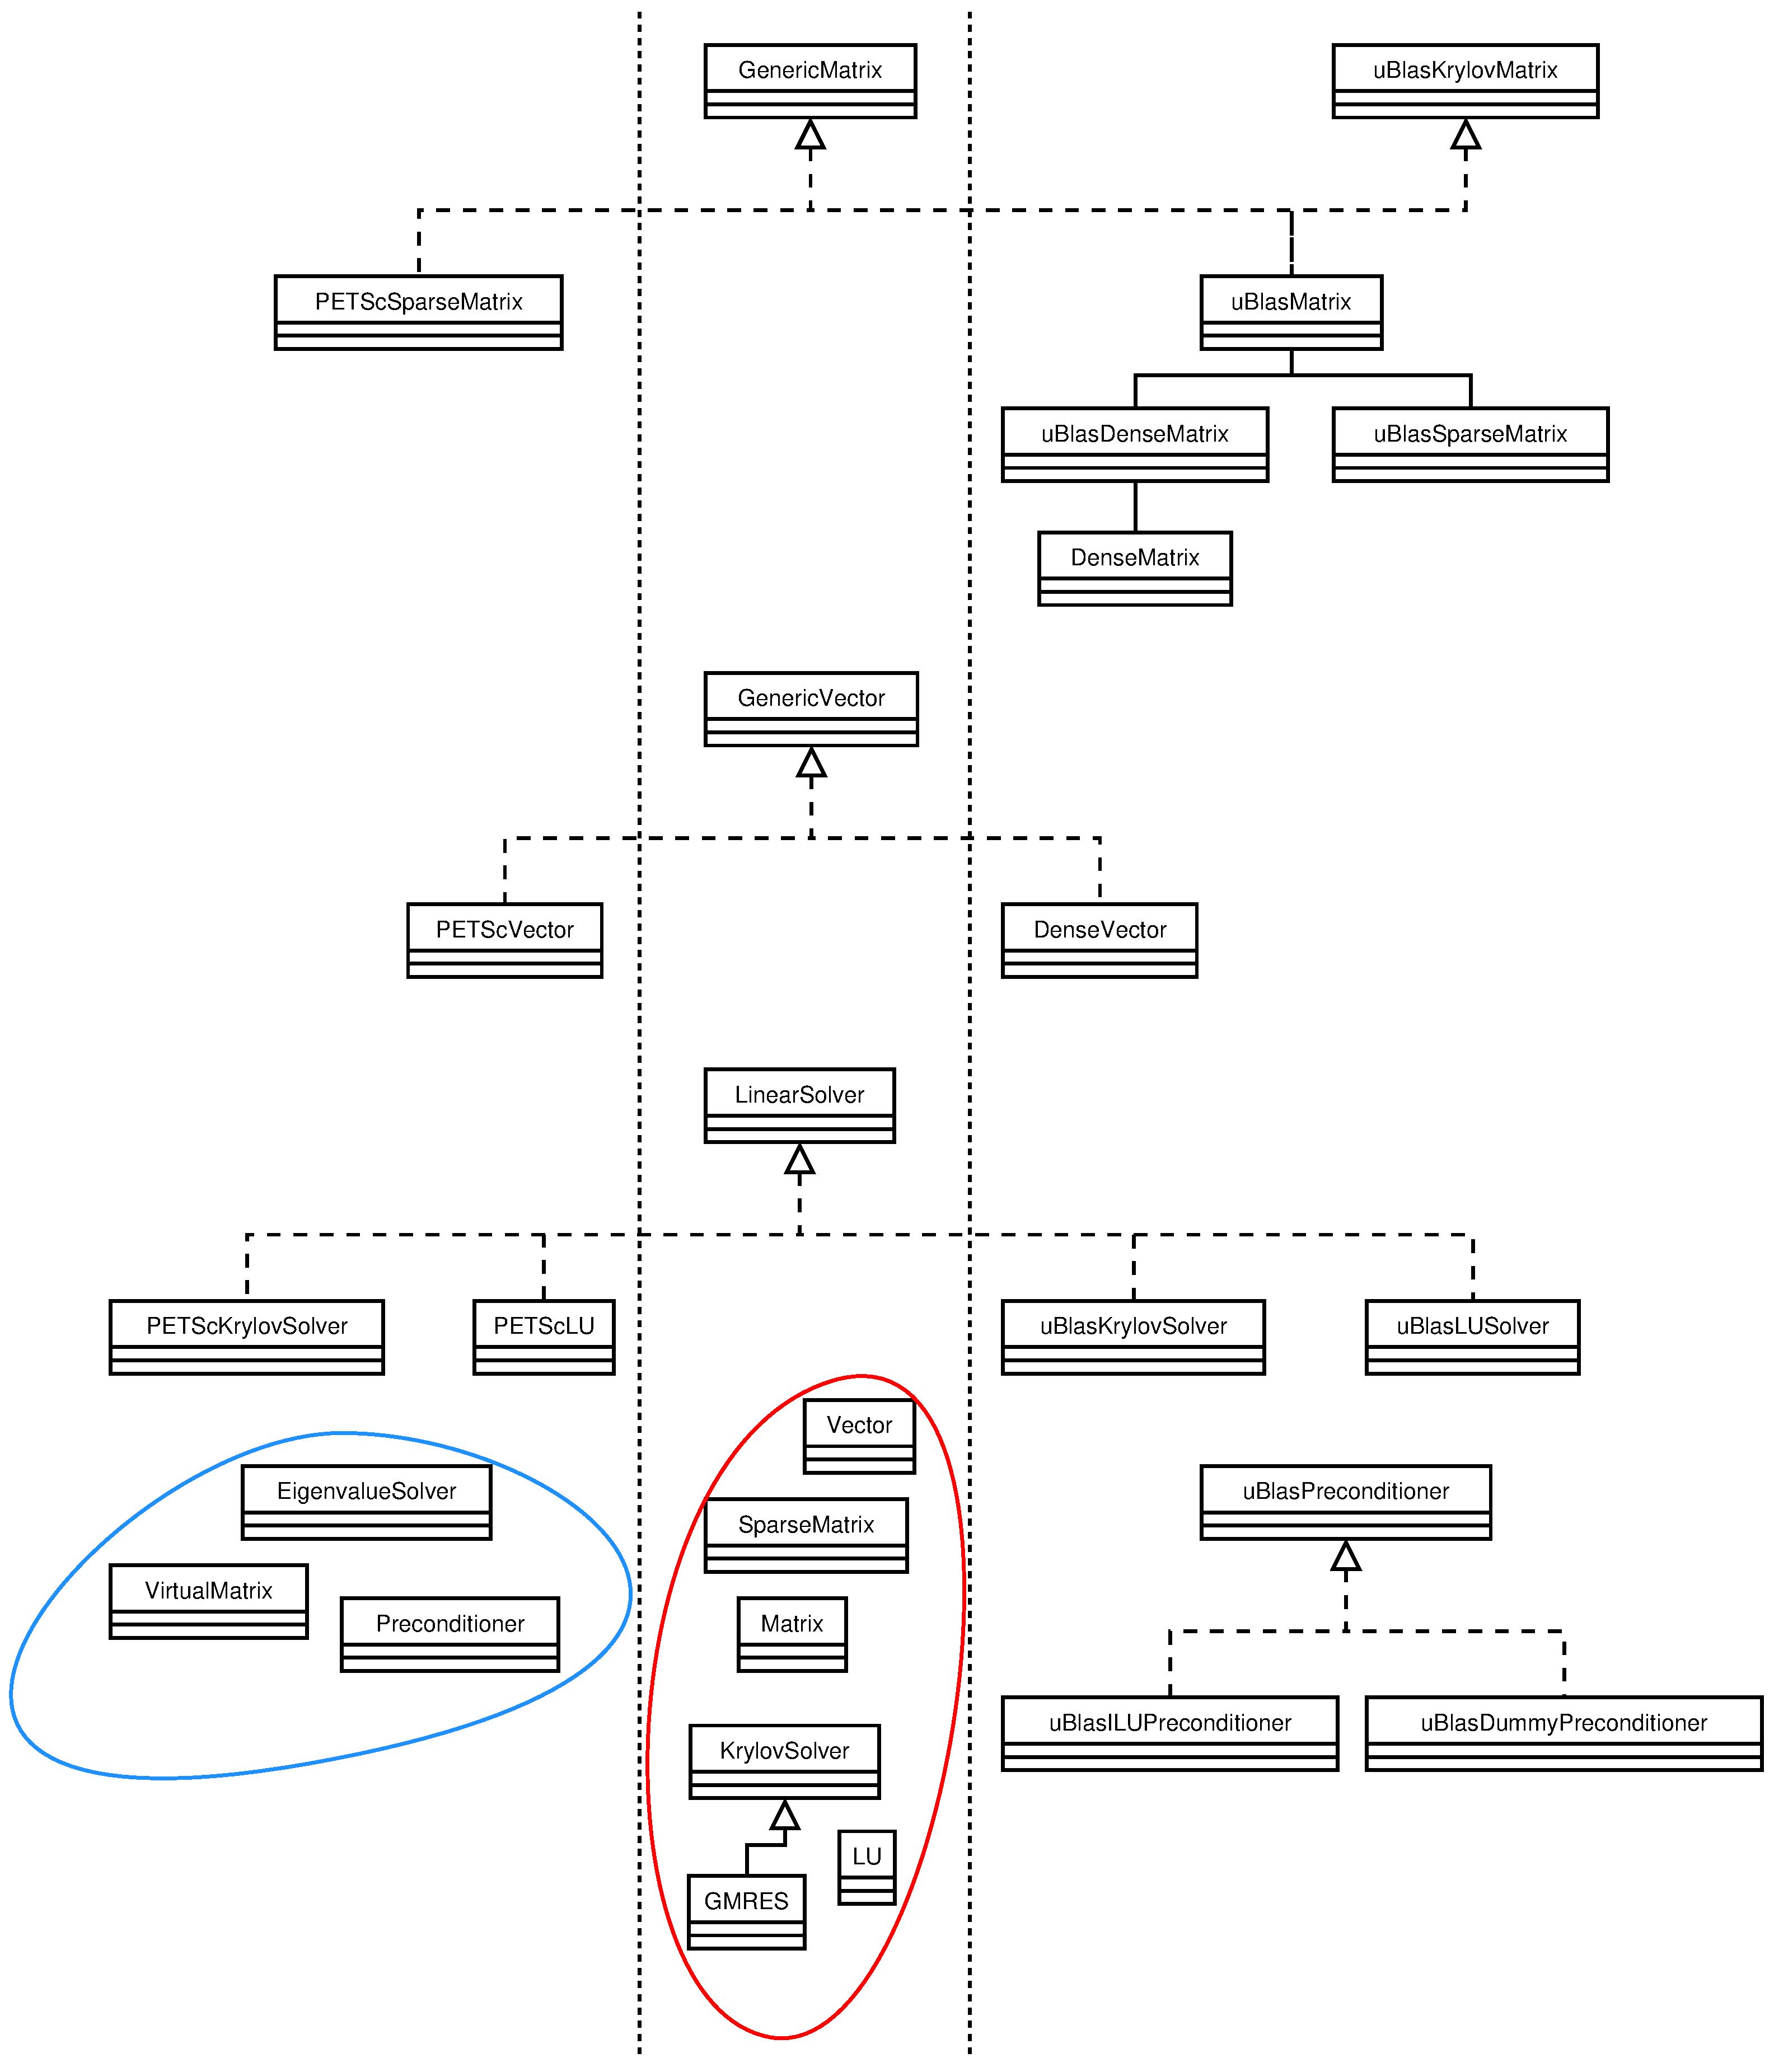
\includegraphics[width=0.95\textwidth]{eps/class-diagram-la.eps}
    \caption{Class diagram of the linear algebra classes in \dolfin{}.}
    \label{fig:laclasses}
  \end{center}
\end{figure}

\section{Matrix-free matrices}

The \dolfin{} class \texttt{VirtualMatrix} represents a matrix-free 
matrix of dimension $M\times M$. 
The matrix-free matrix is a simple wrapper for a PETSc shell matrix. 
The interface is intentionally simple, and for advanced usage the 
PETSc \texttt{Mat} pointer is accessed by the function \texttt{mat()}.  

The class \texttt{VirtualMatrix} enables the use of Krylov subspace
methods for linear systems $Ax = b$, without having to explicitly
store the matrix $A$. All that is needed is that the user-defined
\texttt{VirtualMatrix} implements multiplication with vectors. 
Note that the multiplication operator needs to be defined in terms of
PETSc data structures (\texttt{Vec}), since it will be called from PETSc.

\section{Linear solvers}

A general interface to all linear solvers for systems of the form 
$Ax=b$ is provided through the class \texttt{LinearSolver}. 

In particular, wrappers for a direct LU solver and an iterative 
Krylov GMRES solver are implemented in the classes \texttt{LU} and \texttt{GMRES}. 

To solve the linear system $Ax=b$ using GMRES in \dolfin{}, simply write:  
%
\begin{code} 
Vec x;
GMRES solver; 
solver.solve(A,x,b);
\end{code} 
%


\section{Preconditioning}

The \texttt{Preconditioner} class specifies the interface for user-defined 
Krylov method preconditioners. To implement our own preconditioner we only 
need to supply a function that approximately solves the linear system given 
a right-hand side.

To change the default preconditioner in the \dolfin{} GMRES solver, edit the 
constructor of the \texttt{GMRES} class. For example, to choose the 
ILU preconditioner for GMRES we write 
%
\begin{code}
PC pc;
KSPGetPC(ksp, &pc);
PCSetType(pc, PCILU);
\end{code}

As a complement to the preconditioners available in PETSc, 
\dolfin{} also uses Hypre \cite{www:hypre}, which is a 
library for solving large, sparse linear systems of equations on 
massively parallel computers. 

To use a preconditioner from Hypre together with a PETSc solver in \dolfin{}, we write:  
%
\begin{code}
PCSetType(pc, PCHYPRE );
PCHYPRESetType(pc,"boomeramg");
\end{code}

In particular, the above preconditioner \texttt{boomeramg} is an algebraic multigrid 
preconditioner, which is very useful. 


\section{Eigenvalue solvers}

\dolfin{} also provides wrappers for an eigenvalue solver\index{eigenvalue solver} 
when PETSc is configured and SLEPc \cite{www:slepc} is installed.

The zeroth eigenpair for the problem 
\begin{equation}
  Ax = \lambda x
\end{equation}
can be computed by the following code
\begin{code} 
PETScEigenvalueSolver esolver; 
esolver.solve(A);

real xr, xc;
PETScVector r, c;
getEigenpair(xr, xc, r, c, 0);
\end{code} 
%
The real and complex components of the eigenvalue are returned in \texttt{xr}
and \texttt{xc}, respectively, and the real and complex parts of the eigenvector
are returned in \texttt{r} and \texttt{x}, respectively.

For the generalied eigenvalue problem
\begin{equation}
  A x = \lambda B x,
\end{equation}
%
the second eigenpair can be computed by the following code
%
\begin{code} 
PETScEigenvalueSolver esolver; 
esolver.solve(A, M);

real xr, xc;
PETScVector r, c;
getEigenpair(xr, xc, r, c, 2);
\end{code} 











